% Online scheduling extension; matches the measured batch and feature schedulers.
\begingroup
\color{blue}
\subsection{Reordering Training Tasks for Co-Existing with Foreground Inference Tasks}
\label{subsec:reorder}

Different proxy networks take different amounts of time to process a batch.
When foreground inference runs periodically, background training must fit between requests.
FIFO waits if the next batch cannot finish in the remaining time, even when a later batch could fit.
Reorder uses this gap by running a suitable later task first.
It changes which task starts next; it does not interrupt a task that is already running.

\noindent\textbf{Choosing the next batch.}
Without feature caching, each task is a complete training batch.
Before starting one, we wait for any due foreground requests to finish.
We calculate the time left before the next request and subtract a small safety margin.
We first check the oldest waiting batch.
If its estimated runtime fits, we run it, just as FIFO would.
Otherwise, we look ahead through a limited number of waiting batches.
For each proxy, we consider only its earliest waiting batch, keeping batches for the same proxy in order.
Among the candidates that fit, we choose the one with the longest estimated runtime, using the earlier batch to break ties.
This aims to use as much of the gap as possible.
If no candidate fits, we wait and check again.

Figure~\ref{fig:reorder-example} shows three batches, A, B, and C, that use different proxies and need 15\,ms, 10\,ms, and 5\,ms, respectively.
The available training budget before foreground inference is 20\,ms.
Both methods first run A, leaving 5\,ms.
FIFO then waits because B cannot fit, whereas Reorder runs C in the remaining time.
After foreground inference, FIFO still needs to run B and C, while Reorder only needs to run B.
These durations illustrate the selection rule.

\begin{figure}[!t]
    \centering
    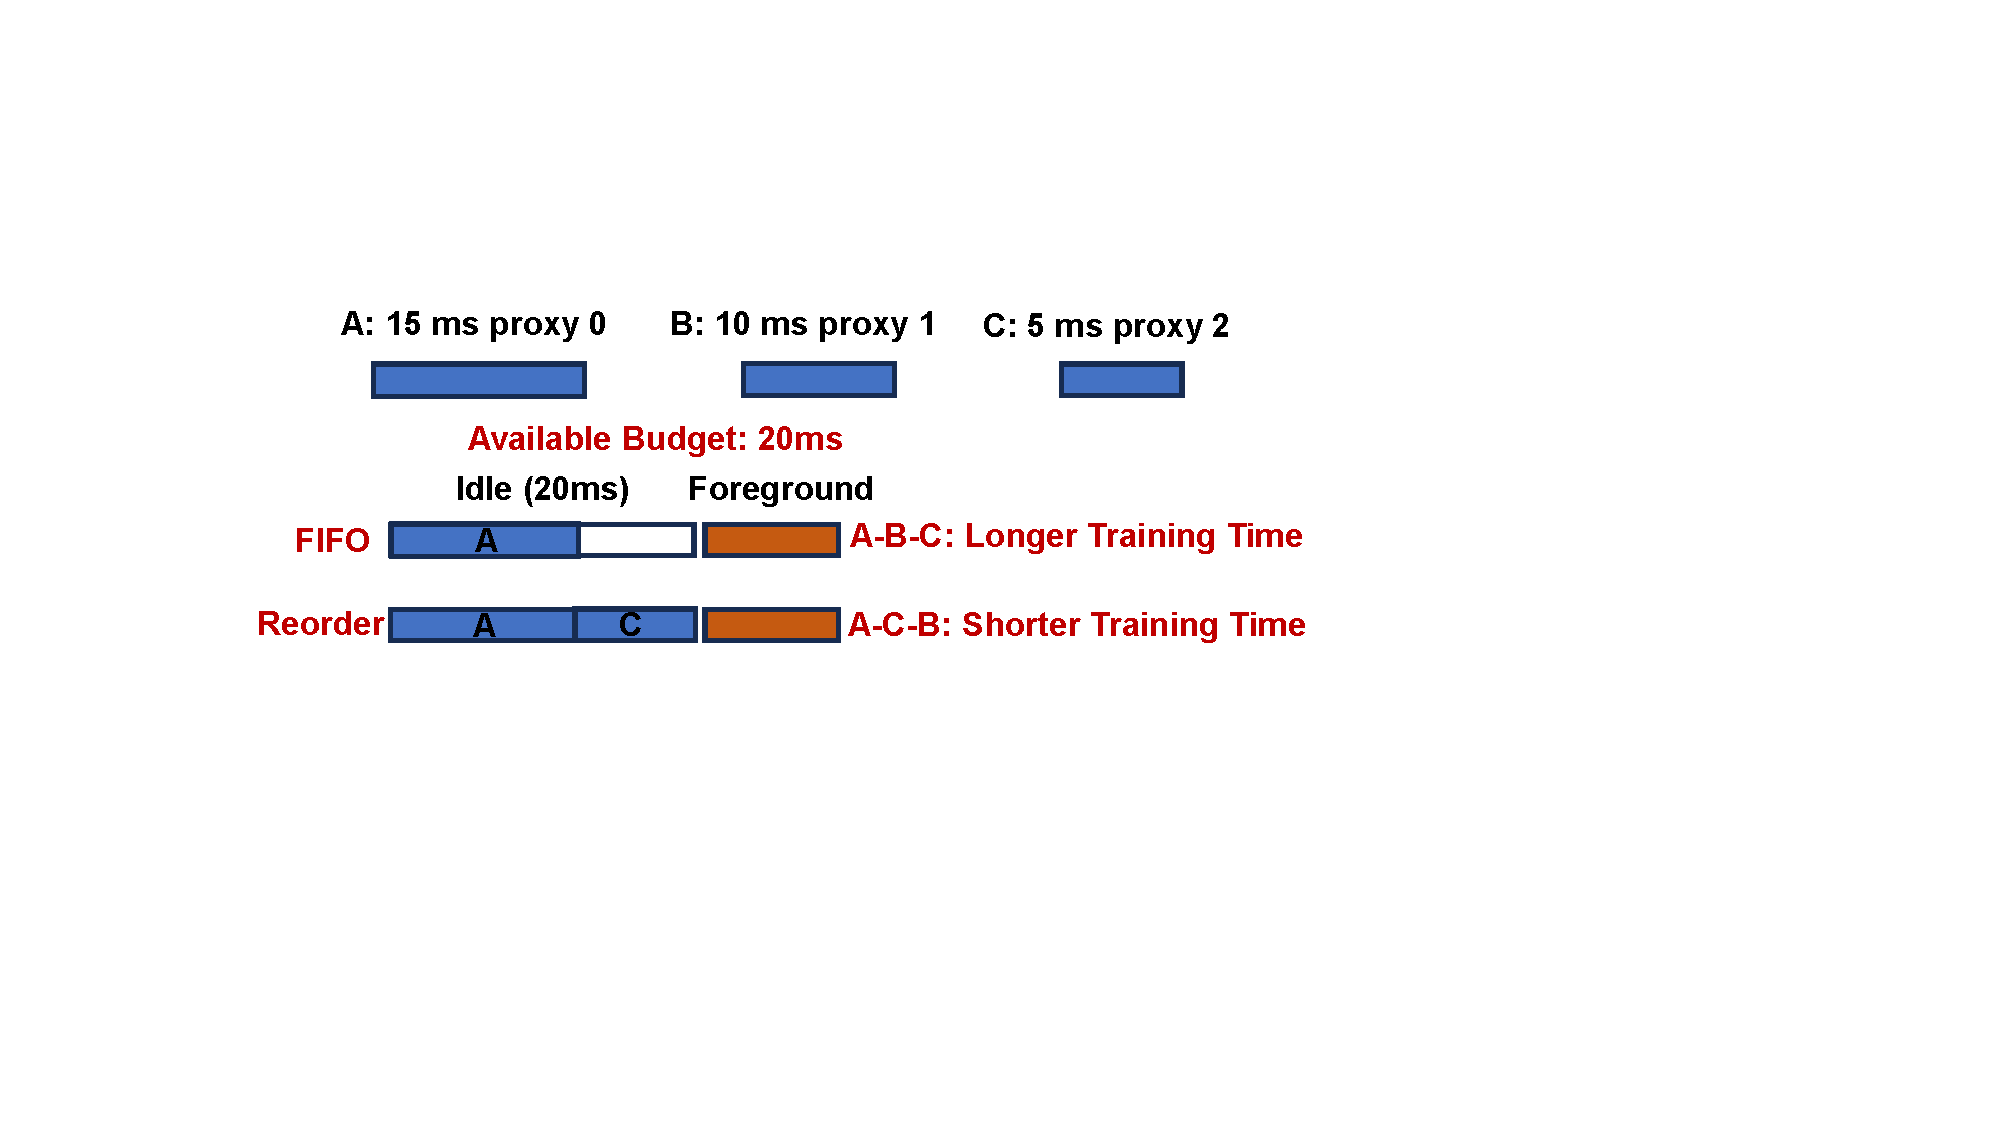
\includegraphics[width=0.98\columnwidth,pagebox=cropbox]{figures/reorder_piebridge.pdf}
    \caption{\textcolor{blue}{An example of FIFO and Reorder with a 20\,ms training budget between foreground inference requests. After A finishes, FIFO leaves 5\,ms unused because B cannot fit. Reorder uses this time to finish C, leaving less training work for the next window. Durations are illustrative.}}
    \label{fig:reorder-example}
\end{figure}

\noindent\textbf{Keeping batches from waiting too long.}
We count how often later batches run ahead of each waiting batch.
Once the oldest batch reaches a preset limit, we stop letting other batches pass it and wait until it fits.
Runtime estimates come from measurements and are updated as training proceeds.
For a complete training batch, the estimate reserves time for a full backward update before the loss-based decision is known.
Section~\ref{subsec:orin-periodic} gives the settings used in our experiments.

% Online-only extension; implementation and protocol in ../orin_scheduling/.
\begingroup
\color{blue}
\subsubsection{Feature Caching}
\label{subsec:feature-prefetch}

An idle gap between foreground requests may be too short for a complete training batch, but long enough for its frozen forward computation.
We cache the output just before the first trainable layer to schedule these two parts separately.
The frozen forward computation can finish in one gap, and training from the first trainable layer can resume in a later gap using the stored features.
We let each admitted operation finish without interrupting it.

The cache is a temporary buffer within one epoch.
It starts empty, and each feature is consumed once and then released.
The next epoch recomputes features even for the same sample and proxy.
Thus, caching does not remove forward computations through reuse across epochs; it allows their results to wait until the remaining training work can run.

Caching also allows us to prepare features for later batches.
For a fixed input and proxy, the frozen output does not depend on the current trainable parameters.
We can therefore reorder feature computations while keeping the work from the first trainable layer onward in the original batch order.
The original sampler sets the batch plan at the start of each epoch, and subsequent loss calculations, update decisions, and sampler feedback use the current parameters and loss history.

If the next batch's features are ready, its remaining training work takes priority; if that work cannot fit, we wait.
Otherwise, we first try to compute its missing features.
If they cannot fit, we look ahead and choose the longest fitting feature computation for another proxy.
We use a fixed-capacity buffer and reserve space for the earliest missing batch.
We admit each operation only when its estimated runtime fits before the next foreground request.
The cache stores features computed ahead of time, while Reorder chooses which ones to prepare.
Its scheduling benefit comes from using gaps that would otherwise be left idle.
Grouping batches that share a proxy can additionally improve forward efficiency, a benefit that does not require foreground inference.
Offline proxy generation and policy training stay unchanged.

\par
\endgroup

% Combined online loop, checked against prefetch_policy.py and
% prefetch_training_benchmark.py. The algorithm describes one training epoch.
\begingroup
\color{blue}
\subsubsection{Combining Feature Caching and Reordering}
\label{subsec:caching-reorder-algorithm}

Algorithm~\ref{alg:caching-reorder} combines the two designs for one epoch.
The original sampler provides the batch order and the proxy for each batch.
The cache $C$ holds features before the first trainable layer, indexed by batch ID; $i$ is the next batch whose remaining training work must run.
The cache starts empty in each epoch, while the trainable parameters and loss history carry over.

\textsc{TrainRest} runs from the first trainable layer using the current parameters.
It keeps the original loss-based update decision, EMA update, and sampler feedback in Algorithm~\ref{alg:on-device_training}.
Its runtime estimate reserves time for a full backward update.
\textsc{FrozenForward} computes only the frozen layers before this point and returns features for each original batch.
Both runtime estimates are updated after the corresponding operation finishes.

\begin{algorithm}[t]
\color{blue}
\footnotesize
\SetAlFnt{\footnotesize\color{blue}}
\SetAlCapFnt{\footnotesize\color{blue}}
\SetAlCapNameFnt{\footnotesize\color{blue}}
\SetNlSty{textbf}{}{}
\SetAlgoNlRelativeSize{-1}
\SetAlgoNoEnd
\SetKw{Continue}{continue}
\SetKwInOut{Input}{Input}
\Input{Ordered batches $Q=(X_j,y_j,p_j)_{j=1}^{M}$; cache capacity $K$ in batches; lookahead $L$; allowed group sizes $S$; safety margin $\delta$; runtime estimates}
\BlankLine
$C\gets\emptyset$; $i\gets 1$\;
\While{$i\le M$}{
    Wait until all due foreground requests finish\;
    $b\gets$ time until next request $-\delta$\;
    \If{$i\in C$}{
        \eIf{estimated runtime of \textnormal{\textsc{TrainRest}}$(i)\le b$}{
            \textsc{TrainRest}$(C[i],y_i,p_i)$\;
            Update its runtime estimate\;
            Release $C[i]$; $i\gets i+1$\;
        }{
            Wait briefly\;
        }
        \Continue\;
    }
    $\mathcal{G}\gets\emptyset$\;
    $W\gets$ uncached batches from $i$ to $\min(M,i+L-1)$\;
    \ForEach{proxy $p$ represented in $W$}{
        $J\gets$ batch IDs in $W$ using $p$, in order\;
        $r\gets K-|C|$\;
        \lIf{$i\notin J$}{$r\gets r-1$}
        $G\gets$ the longest prefix of $J$ with size in $S$, size $\le r$, and estimated forward time $\le b$\;
        \lIf{such a $G$ exists}{$\mathcal{G}\gets\mathcal{G}\cup\{G\}$}
    }
    \If{$\mathcal{G}=\emptyset$}{
        Wait briefly; \Continue\;
    }
    \eIf{a group in $\mathcal{G}$ contains $i$}{
        Select that group as $G$\;
    }{
        Select $G\in\mathcal{G}$ with the longest estimated forward time; break ties by earliest batch ID\;
    }
    $C[G]\gets\textsc{FrozenForward}(Q[G])$\;
    Update the forward runtime estimate for $G$\;
}
\caption{Feature caching with Reorder for one epoch.}
\label{alg:caching-reorder}
\end{algorithm}


When batch $i$ is cached, its remaining training work takes priority.
Otherwise, we prepare features for it if they fit, or use the gap for a later group.
Each group uses one proxy and takes the earliest uncached batches for that proxy within the lookahead range.
We keep the largest allowed group that fits both the time budget and the cache; a group that excludes $i$ must leave one cache slot free for it.
Only feature computation can move ahead: $i$ always advances in the original order, and each cached batch is released after use.
\par
\endgroup

\par
\endgroup
